% SPDX-FileCopyrightText: 2026 Shayan Abrar
% SPDX-License-Identifier: MIT
% Neurocomputing adaptation. Editorial revision of 27 October 2026 (imported from the handoff package, see
% IMPORTED_FROM_PACKAGE.sha256) with the evidence of the research-strengthening revision integrated.
% Not submitted. The journal-specific OSP template and fee conditions remain to be confirmed.
\documentclass[preprint,12pt]{elsarticle}
\usepackage[T1]{fontenc}
\usepackage{lmodern}
\usepackage{microtype}
\usepackage{amsmath,amssymb,booktabs,tabularx,array}
\usepackage[hyphens]{url}
\usepackage[hidelinks,pdfusetitle=false]{hyperref}
\hypersetup{pdftitle={LunarLab: Auditable reward-design experiments in reinforcement learning},pdfauthor={Shayan Abrar}}
\usepackage{placeins}
\newcommand{\lunarlab}{LunarLab}
% Software identity of this revision (the last commit that changed code) and its CI run; see BUILD.md.
\newcommand{\swrev}{c9b9384}
\newcommand{\cirun}{40712412847}
\newcolumntype{Y}{>{\raggedright\arraybackslash}X}
% The figures are tall: let them share a page with text, or fill a float page, near their first mention.
\renewcommand{\topfraction}{0.9}
\renewcommand{\bottomfraction}{0.8}
\renewcommand{\textfraction}{0.07}
\renewcommand{\floatpagefraction}{0.7}
\journal{Neurocomputing}
\biboptions{sort&compress}
% A prepared manuscript is not a submitted manuscript: use a plain title footer.
\makeatletter
\let\ps@pprintTitle\ps@plain
\makeatother
\begin{document}
\begin{frontmatter}
\title{LunarLab: Auditable reward-design experiments in reinforcement learning}
\author[aiub]{Shayan Abrar\corref{corresponding}}
\ead{shayanabrar7@gmail.com}
\cortext[corresponding]{Corresponding author.}
\affiliation[aiub]{organization={American International University-Bangladesh (AIUB)},
addressline={408/1 (Old KA 66/1), Kuratoli, Khilkhet},city={Dhaka},postcode={1229},country={Bangladesh}}
\begin{abstract}
Reward-design experiments need evidence linking the optimized reward, the selected policy and its task behavior. LunarLab is an MIT-licensed research toolkit that connects these stages through named reward decomposition, validation-based checkpoint selection, protected final-test artifacts and behavioral diagnostics. Built on Stable-Baselines3 and Gymnasium, it records original and training rewards separately and associates evaluations with configurations, checkpoint digests and software provenance. Command-line, Python and local web interfaces serve LunarLander-v3, and an adapter-based layer applies the same accounting, selection, freezing and artifact checks to other tasks, demonstrated here on CartPole. In an illustrative LunarLander study, a deliberately flawed hover bonus produces no strict pad landings in 500 test episodes despite a mean re-scored training return of 496.3, while the original-reward baseline lands in 97.6\% of episodes. In a prespecified comparison with twelve designed faults and two controls, LunarLab and a separately implemented Stable-Baselines3 reference of the same audit reach identical verdicts and reject every fault before running the policy; a conventional evaluation script attempts none of these checks. A five-seed CartPole study run through the adapter-based layer exposes a reward that pays for failing. Replays distinguish artifact integrity from numerical agreement across platforms.
\end{abstract}
\begin{keyword}
Reinforcement learning \sep Reward shaping \sep Reward exploitation \sep Reproducibility \sep Research software
\end{keyword}
\end{frontmatter}

\section{Motivation and significance}
Reward shaping changes the objective presented to a reinforcement-learning (RL) agent. Improvements in that objective can coexist with poor task behavior, including the exploitation of unintended incentives \citep{skalse2022gaming}. A useful audit therefore needs more than a training-return curve: it must establish which reward components were earned, which policy was selected, and how that policy performed under task criteria that were not replaced by the shaped reward. Evaluation variability and sensitivity to implementation choices further complicate this interpretation \citep{henderson2018matters,agarwal2021precipice}.

LunarLab organizes an audit around three links: the reward specification to recorded reward components, the selection rule to an identified checkpoint, and that checkpoint to held-out task outcomes. Researchers can follow these links when investigating a surprising behavior or re-evaluating a result. Training, validation, protected final testing and behavioral inspection share configurations and artifact records, so the evidence needed to interpret a reward-design experiment is retained across stages. The local interface supports inspection, while command-line and Python interfaces make the workflow available to scripts.

Established packages supply many of the necessary components. Stable-Baselines3 (SB3) provides tested algorithms, monitoring and evaluation callbacks \citep{raffin2021sb3}. RL Baselines3 Zoo adds configured experiments, tuning and plotting \citep{raffin2020zoo}; CleanRL emphasizes inspectable single-file implementations \citep{huang2022cleanrl}. The imitation library preserves original rewards when replacing them and implements preference learning \citep{gleave2022imitation}. The statistical recommendations underlying rliable motivate robust aggregation across training runs \citep{agarwal2021precipice}, while AI Safety Gridworlds explicitly separates reward from performance measures \citep{leike2017gridworlds}. LunarLab builds on these capabilities, using SB3 as its learning backend and retaining the reward, selection and outcome evidence together. A competent researcher can assemble the same checks with these tools and custom code; Section~\ref{sec:comparison} measures what such an assembly requires and whether it reaches the same verdicts. The software contribution lies in making this connected audit available through a documented, inspectable and tested workflow.

\section{Software description}
\subsection{Architecture and access}
The Python research core uses Gymnasium environments \citep{towers2025gymnasium} and contains reward functions, training and evaluation, artifact handling and analysis (Fig.~\ref{fig:architecture}). A FastAPI service and React/TypeScript client expose local experiment management, telemetry and replay for LunarLander; a three-dimensional view reconstructs the underlying two-dimensional simulation. File-based artifacts and local storage connect the interfaces without a hosted account. Table~\ref{tab:metadata} identifies the implementation described here. The software includes tutorials, Python and HTTP API documentation, extension guidance, issue templates and automated tests.

\begin{figure}[!tbp]
\centering
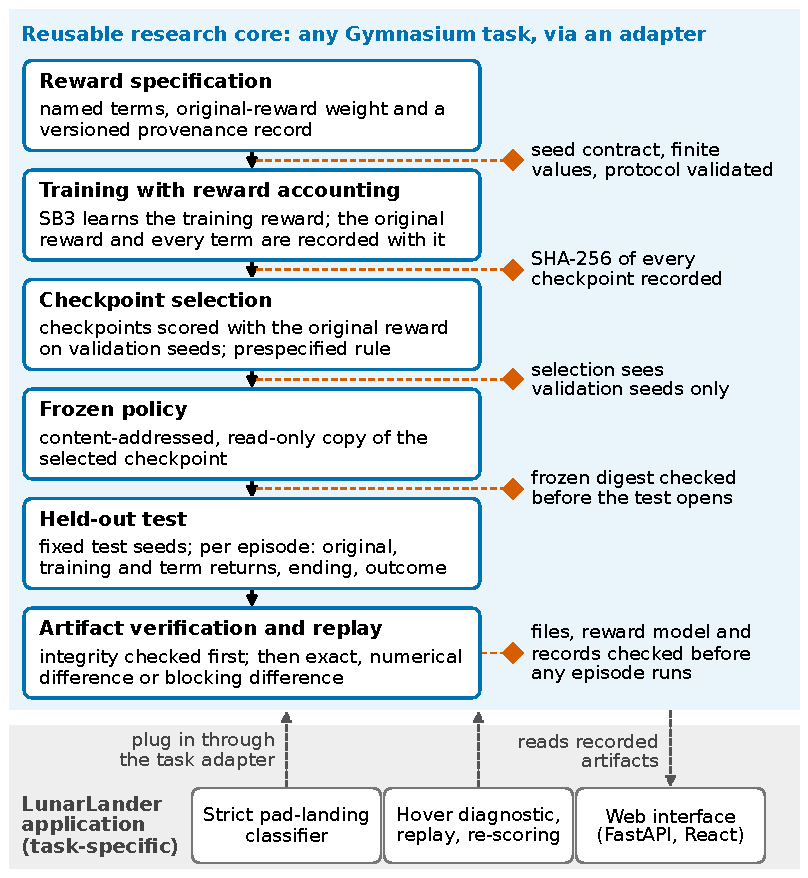
\includegraphics[width=\linewidth]{figures/architecture.pdf}
\caption{Evidence flow and implementation boundaries. Boxes are stages of the reusable research core; solid arrows pass data between stages along the functions named in the figure's source manifest, each checked to exist in the code. Diamonds mark checks that must pass before the next stage. The LunarLander application (dashed arrows) supplies outcome definitions and diagnostics through the task adapter and reads recorded artifacts; the core does not need it.}
\label{fig:architecture}
\end{figure}

\begin{table}[!tbp]
\caption{Software identity and access for the implementation examined in this paper.}
\label{tab:metadata}
\centering\small
\begin{tabularx}{\linewidth}{@{}p{0.25\linewidth}Y@{}}
\toprule
Item & Description \\
\midrule
Software & LunarLab, version 0.1.0, revision \texttt{\swrev} \\
Repository & \url{https://github.com/SHAYAN-ABRAR/lunarlab} \\
License & MIT; component notices are included in the repository \\
Languages & Python; TypeScript/JavaScript for the web application \\
Main dependencies & Gymnasium, Stable-Baselines3, PyTorch, NumPy, FastAPI \\
Supported systems & Windows and Linux; continuous integration includes Python 3.12 and 3.13 \\
Interfaces & Command line, Python API and local web application \\
Documentation & Repository \texttt{README.md}, \texttt{docs/} and executable examples \\
Support & Repository issue tracker; \href{mailto:shayanabrar7@gmail.com}{\texttt{shayanabrar7@gmail.com}} \\
\bottomrule
\end{tabularx}
\end{table}

\subsection{Reward accounting and behavioral criteria}
For a transition from $s_t$ to $s_{t+1}$ under action $a_t$, the training reward is
\begin{equation}
 r_t^{\mathrm{train}}=w\,r_t^{\mathrm{orig}}+\sum_{k=1}^{K}F_k(s_t,a_t,s_{t+1}).
 \label{eq:accounting}
\end{equation}
A configuration specifies the original-reward weight $w$ and named additional terms $F_k$. Shared pure functions implement each term for training, evaluation and trajectory re-scoring, avoiding separate definitions of the same reward. The wrapper preserves observations and episode-ending signals. It refuses a non-finite original reward, term output or weight, and finite values whose episode total would overflow, naming the quantity; the failed episode yields no summary, and further steps are refused until a reset. An episode summary is therefore emitted only when every value the wrapper checks for that episode is finite. Episode records store original return, training return and component totals; transition traces are optional. A versioned provenance record identifies the reward definition by a full SHA-256 digest of its declared description and, separately, by the digest and repository status of each implementing source file, a digest of each implementing function's own source and the values it captures. A description digest cannot identify what code computes, and the record does not fingerprint every dependency: imported modules, module-level data and library versions lie outside it, and two lambdas on one source line with equal captured values are indistinguishable. Code typed into an interactive session, or a captured value without a JSON form, is reported as incompletely identified. Original return remains an environment-defined reference, and behavioral criteria provide a separate account of task completion.

LunarLander can terminate with an at-rest outcome away from the intended pad. LunarLab therefore distinguishes that outcome from a strict pad landing. The latter requires an at-rest termination, no body contact during the episode, recorded leg contact, both leg bodies horizontally between the pad flags, and a final absolute angle at most 0.35 radians. The classifier records which conditions fail and versions its category definitions. It uses leg contact observed during the episode because final-frame contact flags can be cleared when contacts move between terrain fixtures. This explicit operational definition makes a landing claim inspectable beyond the environment's terminal reward.

Built-in rewards include a per-step penalty, a deliberately flawed hover bonus and potential-based shaping. The potential term is
\begin{equation}
 F_{\Phi}(s_t,s_{t+1})=\alpha\bigl[\gamma\Phi(s_{t+1})-\Phi(s_t)\bigr],
 \label{eq:potential}
\end{equation}
with the learner's discount $\gamma$. True termination uses an absorbing-state potential of zero, also when the time limit is reached on the same step; time-limit truncation alone uses the actual final observation, consistent with value bootstrapping. Tests check these cases and the discounted telescoping identity against sums calculated by hand on a small deterministic environment. The policy-invariance result for appropriate potential transformations \citep{ng1999shaping} concerns the objective under its assumptions; finite-budget learning can still differ.

\subsection{Checkpoint selection and artifact provenance}
The protocol validates environment settings and requires validation and test seeds to be non-empty lists of nonnegative integers, without duplicates and without overlap; booleans, floats and numeric strings are refused rather than converted. Mean original return on validation seeds selects the checkpoint. On first final testing, the selected checkpoint is copied to a protected artifact with a SHA-256 digest; interrupted evaluations reuse that copy. Configurations, protocol hashes, transition counts and software records accompany the results. A test-exposure registry marks derived experiments as exploratory, although it cannot prevent an investigator from using knowledge gained from earlier tests.

Continuation restores learning state, including networks, optimizer state and counters. DQN continuation also restores its replay buffer and associated metadata. Simulator state and all random-number streams are not restored, so an interrupted run need not follow the trajectory of an uninterrupted run. Likewise, a digest establishes file identity rather than numerical reproducibility. Exported learned-reward policies include the original reward-model parameters and metadata, and integrity checks reject missing or corrupt dependencies before evaluation.

\subsection{An adapter-based audit layer}
The principal training, checkpoint and web workflows target discrete-action LunarLander-v3. A separate \texttt{lunarlab.audit} layer accepts task adapters that define outcomes, metrics, diagnostics and reward-term factories. Through it, the reward accounting, seed and finite-value contracts, provenance record, fixed-seed policy audit, checkpoint selection, freezing (the same function the main pipeline uses), digest-checked final test, artifact export and verified replay are available to any task with an adapter. Adapters exist for LunarLander-v3 and CartPole-v1, the two tasks on which the layer is demonstrated; policies are audited through a function from observation to action, and the study workflow trains with PPO from SB3. A prespecified study protocol fixes the designs, learner, seeds and selection rule before training. A command (\texttt{lunarlab audit-artifact verify|reproduce}) checks an exported artifact before any episode runs. Learner seeds and environment seeds are recorded separately: SB3 re-seeds the environments when a model is built, so the layer sets the training environments' first-reset seeds afterwards and verifies them, while later training episodes continue each environment's random stream. Extending the complete application would additionally require generalizing run configuration, environment construction, episode schemas and the interface components.

\section{Illustrative reward-design audit}
\subsection{Experimental protocol}
The primary demonstration compares four reward designs using PPO \citep{schulman2017ppo} with training seeds 0--4. All use calm, default LunarLander physics and the same policy architecture and optimizer settings. The configured budget is one million transitions; rollout batching gives 1,003,520 actual transitions per run. Separate policy and value networks each have two 64-unit tanh layers. Four environments collect 1,024 steps each per rollout; optimization uses minibatches of 64, four epochs, learning rate $3\times10^{-4}$, discount 0.999 and generalized-advantage parameter 0.98. The saved configurations provide the remaining settings.

Checkpoint selection uses ten validation seeds, 10,000--10,009. Each selected policy is evaluated deterministically on the same 100 held-out seeds, 20,000--20,099, with a 1,000-step episode limit. The original-reward baseline adds no reward term. The time penalty subtracts 0.01 per step. The hover design adds 1.0 when the next observation lies in its configured band: normalized height 0.25--1.0, absolute angle at most 0.2, absolute horizontal and vertical velocities at most 0.1, and absolute angular velocity at most 0.2. The potential design uses $\alpha=10$ and a bounded negative potential combining position, speed, attitude and angular velocity; its exact weights and function are in the supplied configurations and source.

The unit of aggregation is a trained policy. We report the interquartile mean (IQM) of its 100-episode mean original returns, implemented as a 25\% trimmed mean with integer boundary removal: for five runs, the lowest and highest run means are removed. Percentile intervals use 5,000 bootstrap resamples of training runs. They condition on the fixed evaluation seeds and do not quantify uncertainty from alternative test-seed sets. Five training seeds provide limited precision, so individual policy results remain visible in Fig.~\ref{fig:audit}.

\begin{figure}[!tbp]
\centering
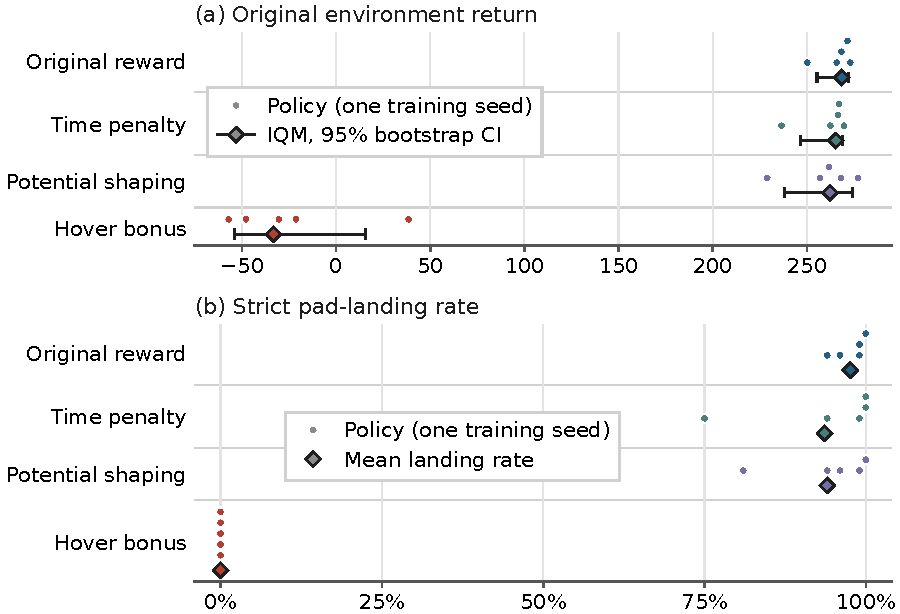
\includegraphics[width=\linewidth]{figures/final_test_audit.pdf}
\caption{Reward-design audit with five trained PPO policies per design and 100 final-test episodes per policy. Circles show policy means in (a) and strict landing rates in (b); vertical displacement separates overlapping markers and leaves horizontal values unchanged. Diamonds denote the group IQM in (a) and mean landing rate in (b). Bars in (a) are 95\% training-run bootstrap intervals. The five hover policies have identical zero landing rates; all five markers are shown. Zero observed landings does not establish a zero population success probability.}
\label{fig:audit}
\end{figure}

\subsection{Observed reward exploitation}
The original-reward baseline has an IQM original return of 268.6 and 488 strict landings in 500 episodes (97.6\%). Time-penalty and potential-based shaping yield IQMs of 265.3 and 262.3, with landing rates of 93.6\% and 94.0\%. Their bootstrap intervals for probability of improvement over the baseline include 0.5; improvement is not established at this budget.

The deliberately flawed hover design yields IQM original return $-33.1$, zero strict landings in 500 episodes and 400 timeouts. Its mean re-scored training return is 496.3, while its mean original return is $-23.5$. These reward channels have different scales, so their numerical difference alone is not a performance comparison. The joint evidence from reward components, absent strict landings and frequent timeouts shows the intended diagnostic use: sustained payment for an intermediate state can coexist with failure to complete the landing. This is an observed failure of the studied design and configuration; the diagnostic has not been validated as a general reward-exploitation detector.

The broader study contains 38 policies and 3,800 final-test episodes across ten groups. Recomputing the exported episode records recovers all policy means, landing and timeout rates, and all ten group IQMs. Additional DQN runs use shorter training budgets and different settings, so they do not support an algorithm-superiority comparison with PPO. The learned-reward runs use simulated preferences derived from original environment reward, with original reward also used for validation. They demonstrate the preference workflow with access to task-reward information. Supplementary group summaries retain these distinctions rather than pooling the studies into a single comparison.

\section{Evaluation of the audit workflow}
\subsection{Comparison with a conventional and an independent SB3 workflow}\label{sec:comparison}
To test whether the integrated workflow checks anything a competent SB3 user could not, we compared three programs on one common input: a neutral directory holding a frozen CartPole policy, its reward definition and parameter file, its seed protocol, a recorded 100-episode evaluation and a recorded trajectory. W1 is the conventional SB3 evaluation: it loads the model, evaluates the deterministic policy on each test seed in an environment whose innermost \texttt{Monitor} records the original reward, and reports return statistics. W2 implements a written ten-point audit specification in custom code on SB3, Gymnasium and NumPy, without importing LunarLab. W3 maps the same input onto LunarLab's public functions. The specification requires the policy digest, file and dependency digests, recorded protocol, seed contract, finite parameters, reward channels, accounting identity, potential convention at truncation and outcome schema to be checked before the policy runs, followed by a replay classified as exact, a permitted numerical difference on another platform, or a blocking difference. The protocol, fault inventory, fixtures and programs were hashed before any program ran on the fixtures; development used separate fixtures.

The inventory has two controls and twelve faults, each changing one property while every digest that could otherwise catch it is recomputed (Fig.~\ref{fig:comparison}). W2 and W3 produced identical results for every check in all fourteen cases: both accepted the clean control with an exact replay and the cross-platform control as a permitted numerical difference, and both rejected all twelve faults through the targeted check before executing the policy. W1 attempted none of the specification's checks; it evaluated 100 episodes in every case without a warning, including a swapped checkpoint whose returns were indistinguishable from the selected one. The program sizes were 65, 277 and 152 counted lines (non-blank, non-comment, non-docstring); W3's lines map the neutral format onto LunarLab, whose own artifacts are checked by one command. On the clean control, five randomized runs per program had median wall times of 20.9, 21.0 and 21.7~s and peak memory of 288, 289 and 293~MB; run-to-run variation from the machine exceeded the differences, so no cost difference is claimed.

\begin{figure}[!tbp]
\centering
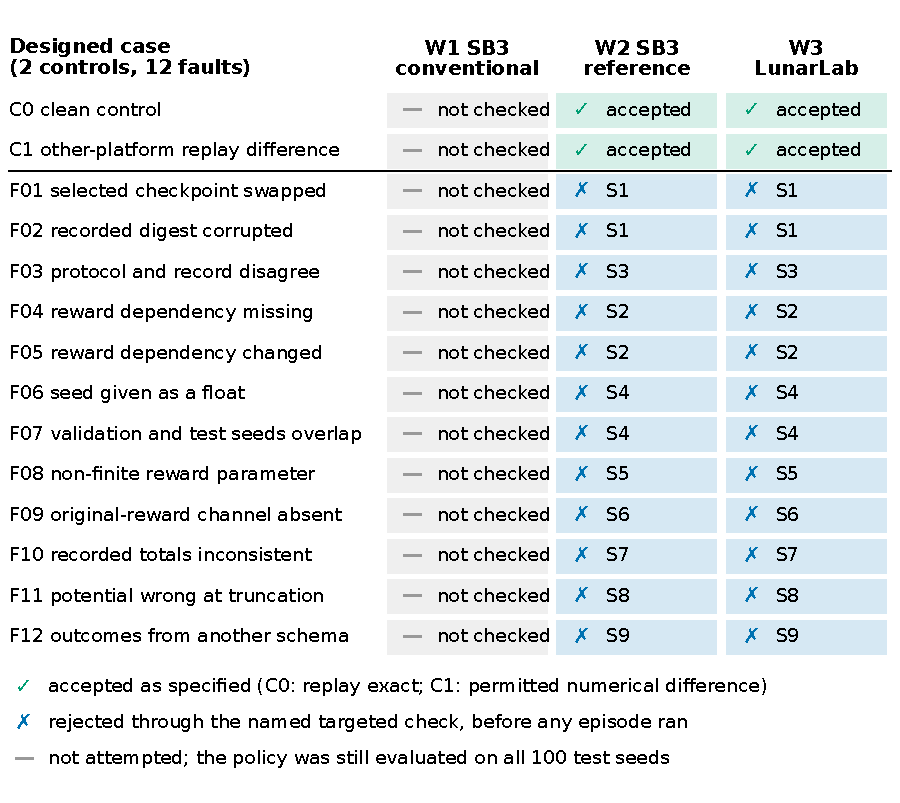
\includegraphics[width=\linewidth]{figures/workflow_comparison.pdf}
\caption{Outcomes of the prespecified fault-injection comparison: fourteen designed cases, each run once by each program. S1--S9 name the specification's integrity checks (policy digest, file and dependency digests, recorded protocol, seed contract, finite parameters, reward channels, accounting identity, potential convention, outcome schema). The results describe these designed cases only; they do not estimate how often such faults occur or the detection of faults outside the set.}
\label{fig:comparison}
\end{figure}

The comparison demonstrates agreement with a separately implemented reference on the prespecified cases and clarifies the contribution: LunarLab supplies these checks as tested library functions, not checks unavailable elsewhere. For LunarLab's own exported artifacts, \texttt{lunarlab audit-artifact verify} runs the equivalents of S1--S7 and S9 before any episode, and \texttt{reproduce} adds the replay classification (S10); the potential-convention check (S8) needs a recorded trajectory, which these artifacts do not carry, and is available as a library function. W3 mapped the neutral fixture format onto these functions. Other entry points run only the checks that concern them; the accounting wrapper, for example, enforces the finite-value and accounting contracts during every episode it wraps. Its limits are a single task, policy and trajectory, and that the same developer, assisted by AI tools, wrote the specification, both audit programs and LunarLab; it measures neither researcher time nor usability.

\subsection{A second task: CartPole}
To exercise the adapter-based layer on a separate controlled problem, we prespecified a CartPole-v1 study \citep{barto1983neuronlike} with three PPO reward designs: the original reward (+1 per step, a 500-step limit counted as success), the adapter's existing upright potential ($\alpha=1$, $\Phi=-|\theta|/12^\circ$), and a deliberately flawed bonus of +1000 on a true termination, which in CartPole means failure. The flawed bonus exceeds the largest possible original return, so any failing episode earns more training return than any successful one; hand calculations and a separately labeled pilot confirmed the payments before the main runs. The learner used RL Baselines3 Zoo's tuned CartPole settings \citep{raffin2020zoo} with seeds 50--54 for every design, 100,000 configured transitions (100,096 after rollout rounding), checkpoints every 10,240 transitions selected on 20 original-reward validation seeds, and 100 held-out test seeds per selected policy, all frozen and digest-checked before the test was opened.

The original and potential designs reached the 500-step limit in every test episode for all ten policies, a ceiling at which the two cannot be distinguished. All five flawed-bonus policies failed after about nine steps (mean original return 9.31, 95\% bootstrap interval over policies 9.22--9.40; no completions in 500 episodes), although their own training return of about 1009 exceeded the 500 earned by a successful policy (Fig.~\ref{fig:cartpole}). Selection on original reward could not recover a useful checkpoint: at all ten evaluated checkpoints of every flawed-bonus run, from the first at 10,240 transitions, the mean original validation return lay between 9.05 and 9.55. The study shows a second use of the layer and a reward conflict the audit records expose; with one simple task and a ceiling effect, it does not establish general applicability.

\begin{figure}[!tbp]
\centering
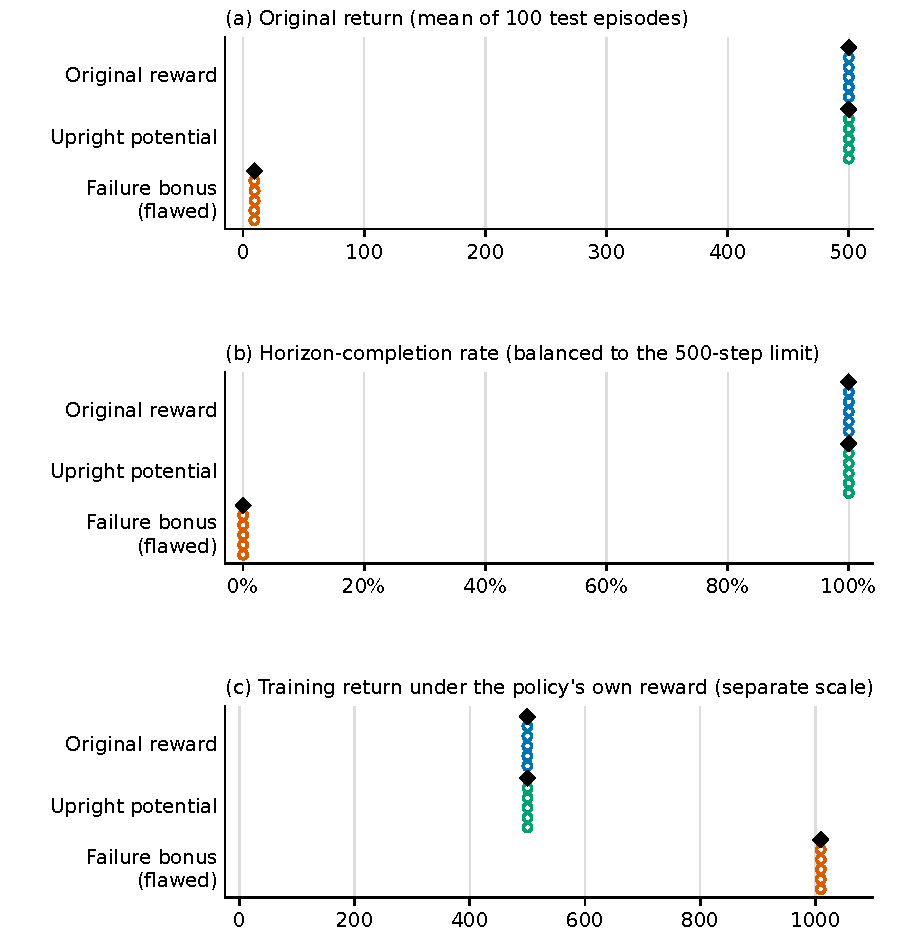
\includegraphics[width=\linewidth]{figures/cartpole_study.pdf}
\caption{CartPole audit, validation-selected policies. Circles are the five trained policies per design (the sampling unit), each the mean over the same 100 held-out test seeds, offset vertically in seed order; diamonds and bars are the mean and 95\% percentile bootstrap interval over policies (10,000 resamples), conditional on those seeds. The widest interval spans 0.17 return units, narrower than a marker, so no bar is visible. Panel (c) uses each design's own training reward and is not comparable with (a).}
\label{fig:cartpole}
\end{figure}

\section{Engineering evaluation and reproducibility}
\subsection{Tests, packaging and execution cost}
At revision \texttt{\swrev}, public continuous integration (run \cirun) records 594 passed Python tests on Linux, four Windows-only skips and 86.04\% combined statement/branch coverage. Targeted Windows jobs pass 293 tests on each of Python 3.12 and 3.13. Browser testing covers 15 flows, and a fresh source-archive installation passes 194 release tests. Tests exercise accounting identities against hand-calculated sums, the seed and finite-value contracts including episode totals that overflow, malformed recorded episodes, protocol validation, checkpoint freezing, continuation, interruption, artifact dependencies and the refusal of thirteen kinds of tampered or malformed artifacts before execution. Runtime reproductions of the seed, finite-value, seeding and reward-identity behavior of the adapter-based layer at preceding revisions found contract gaps that these tests now cover; a subsequent review then found two more, overflowing episode totals and malformed recorded episodes, which this revision corrects without changing any reported result. A deterministic archive builder records the source revision and verifies archive contents; the archive of this revision built on Linux CI and on the recording machine is byte-identical. These checks document specific tested behaviors and supported configurations.

Table~\ref{tab:cost} compares SB3 with a monitoring wrapper, SB3 with LunarLab accounting, and the full LunarLab training workflow. Hyperparameters, training transitions and thread count are matched. The full workflow's loop time is 5.3\% higher, while its additional validation and checkpointing raise elapsed time by 22.1\%. The loop interval includes initialization and excludes separately timed validation and checkpoint operations. Memory is the mean of per-run process peaks measured through training and checkpointing, before optional replay generation. The benchmark records an uncommitted source state based on \texttt{67440c6}; its source manifest is preserved separately from later revisions. The measurements apply to the recorded machine, source state and workload.

\begin{table}[!tbp]
\caption{PPO execution-cost benchmark: 102,400 training transitions per run, three repetitions, Windows 11, Intel i7-13620H and one PyTorch thread. Throughput is mean $\pm$ sample standard deviation; ratios use mean durations. The full workflow performs 18,780 additional validation transitions, taking 7.9 seconds on average. MB denotes $10^6$ bytes.}
\label{tab:cost}
\centering\small
\begin{tabular}{@{}lrrrr@{}}
\toprule
Configuration & Transitions/s & Loop ratio & Elapsed ratio & Peak MB \\
\midrule
SB3 + Monitor & $2{,}158\pm22$ & 1.000 & 1.000 & 310 \\
+ reward accounting & $2{,}115\pm29$ & 1.021 & 1.021 & 310 \\
Full training workflow & $2{,}051\pm55$ & 1.053 & 1.221 & 314 \\
\bottomrule
\end{tabular}
\end{table}

\subsection{Integrity, numerical agreement and behavioral conclusions}
The reproduction workflow reports three distinct forms of evidence. First, digest verification checks that a checkpoint, configuration, recorded evaluation and required reward model match their manifest. All 38 study exports retain the historical checkpoint, configuration and evaluation bytes. This protects the identity of the evidence without predicting the result of a new execution.

Second, re-evaluation compares specified numerical and categorical fields. For three distributed examples---a PPO baseline, PPO hover-bonus policy and DQN baseline---Windows CI and recording-machine evaluations match 300 episodes on length, original return, training return, environment outcome and strict landing status. The six learned-reward policies also match 600 episodes on those fields on the recording machine, starting from an empty data home. Selected-field agreement does not establish identity of every simulator state or training trajectory.

Third, cross-platform reports assess whether the observations motivating an interpretation persist. Linux re-evaluation of the three examples changes numerical results: mean original-return differences are at most 1.52, while individual differences reach approximately 0.28, 11.9 and 192 for the respective policies. Strict landing rates remain 96\%, 0\% and 29\%. On Linux CI, the six learned-reward policies, replayed from an empty data home with their bundled reward models, keep integrity and show numerical differences in every case: per-policy median original-return differences are at most 0.0013 in magnitude, the largest single differences range from 0.007 to 18.3, outcome agreement is 99--100\%, and strict landing rates are unchanged except one policy at 35\% versus 34\% (Fig.~\ref{fig:linux}). Paired tests with Holm correction detect no aggregate difference for any of these policies, but this does not demonstrate statistical equivalence. Nine open-loop trace comparisons of the three examples show early simulator-state differences while greedy actions on recorded observations remain unchanged. This supports a simulator-numerics explanation for the sampled policies and traces without identifying a unique compiler or simulator cause. Evidence from nine policies does not establish cross-platform agreement for the whole study.

\subsection{Reproduction and inspection procedure}
A researcher can begin with the three complete example packages, verify their manifests, re-evaluate a baseline and the hover-bonus policy, and inspect the reported original return and strict landing outcome. The artifact reproduction command reports integrity and re-evaluation status separately. Per-step trace comparisons support more detailed investigation. Recomputing the recorded study summaries requires no retraining. Re-running a policy is a separate operation, and training a new policy adds another source of variability. The CartPole study is rerun from its protocol with one example script, and the comparison from its hashed fixtures. Recomputing the CartPole analysis from its committed run records and rebuilding the figures from the processed results are separate, lighter checks. The accompanying reproduction instructions preserve these distinctions and identify the source revisions and required learned-reward dependencies.

Every figure is produced by a deterministic script: the plots from stored records, and Fig.~\ref{fig:architecture} from a specification whose code references are checked against the source. A manifest records each figure's inputs, plotted values and output digests, and Fig.~\ref{fig:audit}'s plotted values are re-derived from the historical summaries. AI tools assisted the software and figure work. ChatGPT/Codex (OpenAI) assisted software review, the editorial revision and research planning; historical ChatGPT model identifiers were unavailable in the reviewed records. Claude Code (Anthropic) assisted implementation, verification scripts and figure code; retained development metadata identifies Claude Code versions 2.1.283 and 2.1.299 with model identifier \texttt{claude-opus-5-5}, and the code, studies and figures of this revision were prepared with version 2.1.299. The plotted values are read from recorded artifacts rather than generated by a language model.

\section{Research use and limitations}
The hover experiment illustrates the intended research use. A researcher first identifies the incentive paid by the reward term, then verifies which validation-selected checkpoint was evaluated, and finally examines its reward components, strict landing outcomes and timeouts. Re-scoring a trajectory supports inspection of that incentive; artifact verification and re-evaluation test the identity and repeatability of the recorded evidence. These operations make the explanation of a failure inspectable from reward specification through observed behavior, and the CartPole study shows the same chain through the adapter-based layer.

The empirical evidence remains concentrated on LunarLander, with one additional classic-control task that saturates at the configured budget; the adapter-based layer has not been tested on other tasks. Five training seeds per design and fixed evaluation sets limit precision; additional reward designs, budgets and tasks could change the observed rankings. The original environment reward is itself a proxy, and strict landing is a task-specific criterion. The workflow comparison covers designed faults on one task and was not performed by independent users; usefulness to independent research teams remains to be evaluated. Integrity checks cannot eliminate selection bias, investigator reuse of test knowledge or numerical variation across platforms.

\section{Conclusion}
LunarLab links reward specifications to component records, checkpoint selection to protected policy artifacts, and those artifacts to task outcomes. The LunarLander study illustrates how these links support investigation of a reward-design failure, a second task exercises the same links through the adapter-based layer, and a separately implemented reference reaches the same verdicts on the designed faults. Re-evaluation separates file integrity from numerical agreement and behavioral conclusions. The open implementation and exported artifacts make the demonstrated failures and the experimental process available for inspection and reuse.

\FloatBarrier
\section*{Code and data availability}
The MIT-licensed source, documentation, recorded result summaries, three complete example packages and the six learned-reward packages are available at \url{https://github.com/SHAYAN-ABRAR/lunarlab}. The implementation described here is revision \texttt{\swrev} on the review branch \texttt{research/neurocomputing-review-repairs}, which has not yet been merged. It corrects two input-validation defects that a subsequent review found in revision \texttt{30bd3f6}, the previously described revision, which is merged into the main branch; the correction changes no reported result. The experiments ran on recorded source states: the CartPole study on \texttt{e7c3fab}, the workflow comparison on \texttt{5c7a62a} (its LunarLab program, rerun on \texttt{\swrev}, reaches identical verdicts) and the six-policy Linux replay in CI on \texttt{dea292c}, while each LunarLander run records its own revision. Their protocols, raw episode records, comparison outputs, Linux replay reports and figure manifests are under \texttt{reports/neurocomputing-2026-10-27/}, and the repairs' evidence is under \texttt{reports/neurocomputing-review-repairs-2026-10-28/}. The complete 38-policy export, including learned-reward dependencies, is provided in \texttt{LunarLab\_38\_Policy\_Study.zip} with the matching source archive \texttt{lunarlab-0.1.0-444a4c5-src.tar.gz}, and the CartPole study's frozen checkpoints accompany the review package. These accompany this manuscript as supplementary material and have not yet been deposited in a separate public archive; no release or archive identifier exists yet.

\section*{Funding}
This research was self-funded. It received no specific grant from funding agencies in the public, commercial or not-for-profit sectors.

\section*{Declaration of competing interest}
The author declares no competing interests.

\section*{Acknowledgments}
The author thanks American International University-Bangladesh (AIUB) for its institutional support.

% Working draft: disclosure retained separately; restore before journal submission.
% % Preserved separately at the author's request for this working draft.
% Elsevier requires this disclosure in the submitted manuscript.
% Review and finalize author oversight wording, then restore before references using:
% % Preserved separately at the author's request for this working draft.
% Elsevier requires this disclosure in the submitted manuscript.
% Review and finalize author oversight wording, then restore before references using:
% % Preserved separately at the author's request for this working draft.
% Elsevier requires this disclosure in the submitted manuscript.
% Review and finalize author oversight wording, then restore before references using:
% \input{AI_Disclosure_For_Submission}
\section*{Declaration of generative AI and AI-assisted technologies in the manuscript preparation process}
During preparation of this manuscript, the author used ChatGPT/Codex (OpenAI) and Claude Code (Anthropic) for organization, language revision, LaTeX preparation and checks against the available source artifacts. The author retains responsibility for the accuracy, interpretation and final approval of the manuscript.

\section*{Declaration of generative AI and AI-assisted technologies in the manuscript preparation process}
During preparation of this manuscript, the author used ChatGPT/Codex (OpenAI) and Claude Code (Anthropic) for organization, language revision, LaTeX preparation and checks against the available source artifacts. The author retains responsibility for the accuracy, interpretation and final approval of the manuscript.

\section*{Declaration of generative AI and AI-assisted technologies in the manuscript preparation process}
During preparation of this manuscript, the author used ChatGPT/Codex (OpenAI) and Claude Code (Anthropic) for organization, language revision, LaTeX preparation and checks against the available source artifacts. The author retains responsibility for the accuracy, interpretation and final approval of the manuscript.


\appendix
% elsarticle numbers appendix figures A.n but does not reset the counter.
\setcounter{figure}{0}
\section{Cross-platform replay of the learned-reward policies}
\begin{figure}[!htbp]
\centering
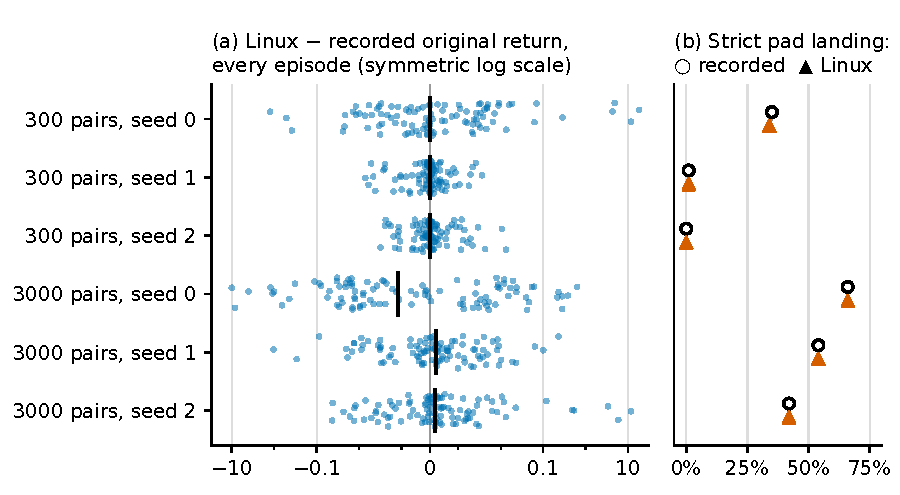
\includegraphics[width=\linewidth]{figures/linux_replay.pdf}
\caption{Linux replay of the six learned-reward policies (CI run 40545198707) against their recording-machine evaluation. (a) Difference in original return for every one of the 100 test episodes per policy, on a symmetric logarithmic axis that is linear within $\pm10^{-3}$; vertical jitter only; bars mark the median. (b) Strict pad-landing rate as recorded and on Linux. Integrity checks passed for every package before any episode ran.}
\label{fig:linux}
\end{figure}
\FloatBarrier

\bibliographystyle{elsarticle-num}
\bibliography{references}
\end{document}
